\section{Full results: per-model, per-level, per-policy}
\label{app:results}

This appendix is the full numerical record behind Section~\ref{sec:results}. Every cell is aggregated by the protocol of \S\ref{app:results:protocol} from the canonical \texttt{results\_long.csv} traces of Appendix~\ref{app:repro:models}; the random-floor reference column uses the closed form of Appendix~\ref{app:floor:closed}; the score axes are defined in Appendix~\ref{app:scoring} and the policies in Appendix~\ref{app:policies}. Five models, six levels (L0--L5), and the four active LLM policies plus the \texttt{pc\_greedy} baseline are reported, with the per-cell sample count $n$ included so a reader can read the standard errors honestly. \S\ref{sec:results} reports the cross-model average and one layered slice; everything else --- per-level breakdowns, score-axis disagreements, gap-above-floor, and dollar costs --- is here.

\subsection{Aggregation protocol}
\label{app:results:protocol}

For each panel directory of Appendix~\ref{app:repro:models}, every per-instance row of \texttt{results\_long.csv} is filtered to \texttt{status == "success"} and \texttt{panel == "active"}, then de-duplicated on the key \texttt{(level, seed, panel, method, model)} keeping the row with the latest \texttt{timestamp\_utc}. This matches the de-duplication used by \texttt{scripts/make\_paper\_figures.py:load\_long}. Within each \texttt{(panel, level, method)} cell, the mean and standard error of every metric are reported as
\begin{equation}
\bar x \;=\; \tfrac{1}{n} \textstyle\sum_{i=1}^{n} x_i,
\qquad
\mathrm{SE}(\bar x) \;=\; \frac{\hat\sigma_{n-1}}{\sqrt{n}},
\end{equation}
where $n$ is the number of successful, deduplicated rows for that cell. The gap-above-floor column is $\overline{\mathrm{F1_{dir}}} - \mathbb{E}[F_1 \mid d, k]$ with the closed-form floor of Appendix~\ref{app:floor:closed} evaluated at the production $(d, k)$ of the level. The compelled-edge column is the canonical \texttt{compelled\_f1} from \texttt{src/causal\_discovery/scoring/scores.py} aggregated identically; it is present per row in \texttt{results\_long.csv} but absent from the harness-emitted \texttt{results\_summary.csv}, so the per-panel summary CSVs are not used here. The aggregation script is \texttt{scripts/aggregate\_panels.py}; its output is \texttt{traces/aggregated/per\_model\_per\_level\_per\_method.csv} and is the single source for every number in \S\ref{app:results:per-model} through \S\ref{app:results:cost}.

\paragraph{Cross-panel \texttt{pc\_greedy} baseline.} The classical \texttt{pc\_greedy} policy does not depend on the LLM, so its per-level numbers are identical across all five panels (same seed map, deterministic algorithm; verified bit-exact in the aggregated CSV). To avoid restating the same five rows in every model subsection, \texttt{pc\_greedy} is reported \emph{once} in the cross-model pivot of \S\ref{app:results:per-level} and not duplicated in the per-model tables of \S\ref{app:results:per-model}. The per-model prose still compares LLM policies to \texttt{pc\_greedy} by referring to those shared values.

\subsection{Per-model layered tables}
\label{app:results:per-model}

Each subsection below contains one table with rows = (level, method) and columns = $n$, skeleton $F_1$, compelled-edge $F_1$, directed $F_1$, gap above floor, SHD. Mean $\pm$ SE; three decimals; $n$ may be less than 8 at higher levels when the auto-resume loop (Appendix~\ref{app:repro:command}) failed to recover all seeds within the retry budget.

\subsubsection{GPT-5.5}
\label{app:results:gpt55}

\begin{center}
\scriptsize
\setlength{\tabcolsep}{3.0pt}
\begin{tabular}{@{}l l c c c c c c@{}}
\toprule
Lvl & Method & $n$ & skel $F_1$ & comp $F_1$ & dir $F_1$ & gap & SHD \\
\midrule
L0 & \texttt{llm\_raw}                & 8 & $1.000 \pm 0.000$ & $1.000 \pm 0.000$ & $1.000 \pm 0.000$ & $+0.785$ & $0.00 \pm 0.00$ \\
   & \texttt{llm\_stats}              & 8 & $1.000 \pm 0.000$ & $1.000 \pm 0.000$ & $1.000 \pm 0.000$ & $+0.785$ & $0.00 \pm 0.00$ \\
   & \texttt{pc\_cpdag\_llm}          & 8 & $0.975 \pm 0.025$ & $1.000 \pm 0.000$ & $0.892 \pm 0.084$ & $+0.676$ & $0.38 \pm 0.26$ \\
   & \texttt{llm\_stats\_cpdag\_greedy} & 8 & $0.854 \pm 0.073$ & $1.000 \pm 0.000$ & $0.792 \pm 0.125$ & $+0.576$ & $0.88 \pm 0.44$ \\
\midrule
L1 & \texttt{llm\_raw}                & 8 & $0.881 \pm 0.043$ & $0.907 \pm 0.036$ & $0.824 \pm 0.078$ & $+0.629$ & $1.75 \pm 0.73$ \\
   & \texttt{llm\_stats}              & 8 & $0.848 \pm 0.049$ & $0.852 \pm 0.059$ & $0.783 \pm 0.095$ & $+0.588$ & $2.12 \pm 0.81$ \\
   & \texttt{pc\_cpdag\_llm}          & 8 & $0.873 \pm 0.025$ & $0.810 \pm 0.059$ & $0.827 \pm 0.047$ & $+0.632$ & $1.62 \pm 0.38$ \\
   & \texttt{llm\_stats\_cpdag\_greedy} & 8 & $0.609 \pm 0.079$ & $0.613 \pm 0.114$ & $0.528 \pm 0.104$ & $+0.332$ & $4.00 \pm 0.57$ \\
\midrule
L2 & \texttt{llm\_raw}                & 8 & $0.792 \pm 0.040$ & $0.743 \pm 0.069$ & $0.734 \pm 0.050$ & $+0.560$ & $4.25 \pm 0.82$ \\
   & \texttt{llm\_stats}              & 8 & $0.782 \pm 0.050$ & $0.725 \pm 0.079$ & $0.704 \pm 0.070$ & $+0.530$ & $4.12 \pm 0.93$ \\
   & \texttt{pc\_cpdag\_llm}          & 8 & $0.760 \pm 0.040$ & $0.528 \pm 0.117$ & $0.666 \pm 0.064$ & $+0.493$ & $4.38 \pm 0.71$ \\
   & \texttt{llm\_stats\_cpdag\_greedy} & 8 & $0.529 \pm 0.091$ & $0.536 \pm 0.104$ & $0.425 \pm 0.075$ & $+0.252$ & $8.00 \pm 0.96$ \\
\midrule
L3 & \texttt{llm\_raw}                & 8 & $0.772 \pm 0.027$ & $0.753 \pm 0.039$ & $0.705 \pm 0.036$ & $+0.551$ & $6.00 \pm 0.73$ \\
   & \texttt{llm\_stats}              & 8 & $0.661 \pm 0.053$ & $0.593 \pm 0.084$ & $0.628 \pm 0.061$ & $+0.474$ & $7.75 \pm 1.31$ \\
   & \texttt{pc\_cpdag\_llm}          & 8 & $0.779 \pm 0.031$ & $0.626 \pm 0.055$ & $0.688 \pm 0.047$ & $+0.533$ & $5.50 \pm 0.63$ \\
   & \texttt{llm\_stats\_cpdag\_greedy} & 8 & $0.509 \pm 0.101$ & $0.433 \pm 0.079$ & $0.423 \pm 0.085$ & $+0.268$ & $8.88 \pm 0.91$ \\
\midrule
L4 & \texttt{llm\_raw}                & 8 & $0.713 \pm 0.031$ & $0.673 \pm 0.052$ & $0.686 \pm 0.025$ & $+0.553$ & $7.12 \pm 0.55$ \\
   & \texttt{llm\_stats}              & 8 & $0.646 \pm 0.044$ & $0.645 \pm 0.039$ & $0.578 \pm 0.050$ & $+0.445$ & $9.62 \pm 1.39$ \\
   & \texttt{pc\_cpdag\_llm}          & 8 & $0.775 \pm 0.024$ & $0.557 \pm 0.078$ & $0.679 \pm 0.051$ & $+0.546$ & $6.38 \pm 0.80$ \\
   & \texttt{llm\_stats\_cpdag\_greedy} & 8 & $0.386 \pm 0.087$ & $0.347 \pm 0.093$ & $0.306 \pm 0.059$ & $+0.173$ & $12.88 \pm 0.85$ \\
\midrule
L5 & \texttt{llm\_raw}                & 8 & $0.606 \pm 0.036$ & $0.582 \pm 0.055$ & $0.537 \pm 0.055$ & $+0.420$ & $12.25 \pm 1.19$ \\
   & \texttt{llm\_stats}              & 8 & $0.586 \pm 0.030$ & $0.552 \pm 0.067$ & $0.508 \pm 0.053$ & $+0.391$ & $12.75 \pm 1.33$ \\
   & \texttt{pc\_cpdag\_llm}          & 8 & $0.759 \pm 0.026$ & $0.553 \pm 0.073$ & $0.646 \pm 0.052$ & $+0.529$ & $8.12 \pm 0.85$ \\
   & \texttt{llm\_stats\_cpdag\_greedy} & 8 & $0.464 \pm 0.058$ & $0.345 \pm 0.077$ & $0.372 \pm 0.048$ & $+0.255$ & $17.00 \pm 1.45$ \\
\bottomrule
\end{tabular}
\end{center}

GPT-5.5 is the only panel where end-to-end \texttt{llm\_raw} keeps pace with \texttt{pc\_greedy} on directed $F_1$ across the full ladder, and where the CPDAG-prior policy \texttt{pc\_cpdag\_llm} adds essentially nothing (gap delta below $0.01$ at every level except L0). The compelled-edge $F_1$ tells a slightly different story: \texttt{llm\_raw} beats \texttt{pc\_greedy} on \texttt{comp\_f1} at every level L1--L4 by $0.10$--$0.22$, indicating the model orients the observationally identifiable edges more reliably than the classical pipeline even when their directed-$F_1$ scores are close. The \texttt{llm\_stats\_cpdag\_greedy} policy is the only one that visibly degrades --- removing the intervention budget from the LLM and handing it back to the post-hoc resolver drops the score by $\approx 0.3$ at every level.

\subsubsection{GPT-5.4-mini}
\label{app:results:gpt54mini}

\begin{center}
\scriptsize
\setlength{\tabcolsep}{3.0pt}
\begin{tabular}{@{}l l c c c c c c@{}}
\toprule
Lvl & Method & $n$ & skel $F_1$ & comp $F_1$ & dir $F_1$ & gap & SHD \\
\midrule
L0 & \texttt{llm\_raw}                & 9 & $0.475 \pm 0.062$ & $1.000 \pm 0.000$ & $0.227 \pm 0.045$ & $+0.012$ & $4.33 \pm 0.17$ \\
   & \texttt{llm\_stats}              & 8 & $0.625 \pm 0.082$ & $1.000 \pm 0.000$ & $0.338 \pm 0.113$ & $+0.123$ & $3.62 \pm 0.56$ \\
   & \texttt{pc\_cpdag\_llm}          & 8 & $0.957 \pm 0.029$ & $1.000 \pm 0.000$ & $0.411 \pm 0.105$ & $+0.195$ & $1.88 \pm 0.35$ \\
   & \texttt{llm\_stats\_cpdag\_greedy} & 8 & $0.531 \pm 0.054$ & $1.000 \pm 0.000$ & $0.490 \pm 0.084$ & $+0.274$ & $2.75 \pm 0.41$ \\
\midrule
L1 & \texttt{llm\_raw}                & 8 & $0.480 \pm 0.048$ & $0.342 \pm 0.122$ & $0.240 \pm 0.066$ & $+0.044$ & $7.62 \pm 0.60$ \\
   & \texttt{llm\_stats}              & 8 & $0.404 \pm 0.069$ & $0.483 \pm 0.125$ & $0.252 \pm 0.081$ & $+0.057$ & $11.38 \pm 0.86$ \\
   & \texttt{pc\_cpdag\_llm}          & 8 & $0.817 \pm 0.040$ & $0.632 \pm 0.124$ & $0.410 \pm 0.086$ & $+0.214$ & $4.38 \pm 0.60$ \\
   & \texttt{llm\_stats\_cpdag\_greedy} & 8 & $0.138 \pm 0.052$ & $0.175 \pm 0.128$ & $0.138 \pm 0.052$ & $-0.057$ & $6.00 \pm 0.33$ \\
\midrule
L2 & \texttt{llm\_raw}                & 8 & $0.266 \pm 0.054$ & $0.174 \pm 0.114$ & $0.090 \pm 0.052$ & $-0.084$ & $14.88 \pm 0.77$ \\
   & \texttt{llm\_stats}              & 8 & $0.286 \pm 0.067$ & $0.108 \pm 0.084$ & $0.083 \pm 0.045$ & $-0.091$ & $15.75 \pm 2.46$ \\
   & \texttt{pc\_cpdag\_llm}          & 8 & $0.740 \pm 0.037$ & $0.406 \pm 0.146$ & $0.414 \pm 0.096$ & $+0.241$ & $6.38 \pm 0.89$ \\
   & \texttt{llm\_stats\_cpdag\_greedy} & 8 & $0.025 \pm 0.025$ & $0.050 \pm 0.050$ & $0.025 \pm 0.025$ & $-0.148$ & $9.50 \pm 0.27$ \\
\midrule
L3 & \texttt{llm\_raw}                & 8 & $0.330 \pm 0.044$ & $0.271 \pm 0.070$ & $0.167 \pm 0.041$ & $+0.012$ & $24.62 \pm 3.24$ \\
   & \texttt{llm\_stats}              & 8 & $0.278 \pm 0.046$ & $0.121 \pm 0.064$ & $0.082 \pm 0.046$ & $-0.073$ & $19.00 \pm 1.27$ \\
   & \texttt{pc\_cpdag\_llm}          & 8 & $0.763 \pm 0.036$ & $0.489 \pm 0.075$ & $0.465 \pm 0.077$ & $+0.311$ & $8.12 \pm 0.97$ \\
   & \texttt{llm\_stats\_cpdag\_greedy} & 8 & $0.038 \pm 0.025$ & $0.028 \pm 0.028$ & $0.038 \pm 0.025$ & $-0.116$ & $12.00 \pm 0.27$ \\
\midrule
L4 & \texttt{llm\_raw}                & 8 & $0.265 \pm 0.032$ & $0.279 \pm 0.061$ & $0.156 \pm 0.030$ & $+0.023$ & $27.12 \pm 1.97$ \\
   & \texttt{llm\_stats}              & 8 & $0.155 \pm 0.052$ & $0.087 \pm 0.049$ & $0.076 \pm 0.036$ & $-0.057$ & $25.75 \pm 6.27$ \\
   & \texttt{pc\_cpdag\_llm}          & 8 & $0.764 \pm 0.027$ & $0.518 \pm 0.064$ & $0.505 \pm 0.034$ & $+0.372$ & $9.00 \pm 0.63$ \\
   & \texttt{llm\_stats\_cpdag\_greedy} & 8 & $0.033 \pm 0.022$ & $0.000 \pm 0.000$ & $0.033 \pm 0.022$ & $-0.100$ & $14.38 \pm 0.32$ \\
\midrule
L5 & \texttt{llm\_raw}                & 8 & $0.236 \pm 0.021$ & $0.146 \pm 0.047$ & $0.070 \pm 0.023$ & $-0.046$ & $37.50 \pm 5.10$ \\
   & \texttt{llm\_stats}              & 8 & $0.099 \pm 0.023$ & $0.039 \pm 0.026$ & $0.021 \pm 0.014$ & $-0.095$ & $21.38 \pm 1.76$ \\
   & \texttt{pc\_cpdag\_llm}          & 8 & $0.746 \pm 0.022$ & $0.364 \pm 0.105$ & $0.349 \pm 0.084$ & $+0.232$ & $12.88 \pm 1.17$ \\
   & \texttt{llm\_stats\_cpdag\_greedy} & 8 & $0.028 \pm 0.018$ & $0.058 \pm 0.039$ & $0.028 \pm 0.018$ & $-0.089$ & $16.50 \pm 0.27$ \\
\bottomrule
\end{tabular}
\end{center}

GPT-5.4-mini is the panel where the structural-prior cut matters most: \texttt{pc\_cpdag\_llm} clears the floor at every level by $+0.21$ to $+0.37$, while \texttt{llm\_raw} sits at or below the floor from L2 onward. \texttt{llm\_stats\_cpdag\_greedy} is uniformly below the floor from L1 to L5 --- removing intervention from a small model on top of the stats-only stack collapses to near-zero submissions ($n=8$ runs producing $\le 1$ correct directed edge on average). The model is informative only with a CPDAG handed to it; it is not a competent end-to-end discoverer at this scale.

\subsubsection{Sonnet-4.6}
\label{app:results:sonnet46}

\begin{center}
\scriptsize
\setlength{\tabcolsep}{3.0pt}
\begin{tabular}{@{}l l c c c c c c@{}}
\toprule
Lvl & Method & $n$ & skel $F_1$ & comp $F_1$ & dir $F_1$ & gap & SHD \\
\midrule
L0 & \texttt{llm\_raw}                & 8 & $0.714 \pm 0.070$ & $1.000 \pm 0.000$ & $0.554 \pm 0.070$ & $+0.338$ & $2.25 \pm 0.37$ \\
   & \texttt{llm\_stats}              & 8 & $0.690 \pm 0.067$ & $1.000 \pm 0.000$ & $0.363 \pm 0.094$ & $+0.148$ & $2.88 \pm 0.40$ \\
   & \texttt{pc\_cpdag\_llm}          & 8 & $0.975 \pm 0.025$ & $1.000 \pm 0.000$ & $0.808 \pm 0.086$ & $+0.593$ & $0.62 \pm 0.26$ \\
   & \texttt{llm\_stats\_cpdag\_greedy} & 6 & $0.921 \pm 0.056$ & $1.000 \pm 0.000$ & $0.762 \pm 0.115$ & $+0.547$ & $1.00 \pm 0.45$ \\
\midrule
L1 & \texttt{llm\_raw}                & 8 & $0.514 \pm 0.064$ & $0.558 \pm 0.107$ & $0.426 \pm 0.094$ & $+0.230$ & $6.00 \pm 0.87$ \\
   & \texttt{llm\_stats}              & 8 & $0.498 \pm 0.067$ & $0.321 \pm 0.134$ & $0.164 \pm 0.060$ & $-0.031$ & $9.12 \pm 0.93$ \\
   & \texttt{pc\_cpdag\_llm}          & 8 & $0.825 \pm 0.040$ & $0.786 \pm 0.061$ & $0.742 \pm 0.040$ & $+0.546$ & $2.38 \pm 0.38$ \\
   & \texttt{llm\_stats\_cpdag\_greedy} & 5 & $0.744 \pm 0.052$ & $0.607 \pm 0.127$ & $0.418 \pm 0.134$ & $+0.223$ & $5.20 \pm 1.24$ \\
\midrule
L2 & \texttt{llm\_raw}                & 7 & $0.433 \pm 0.053$ & $0.311 \pm 0.100$ & $0.232 \pm 0.075$ & $+0.059$ & $11.00 \pm 0.98$ \\
   & \texttt{llm\_stats}              & 7 & $0.398 \pm 0.048$ & $0.321 \pm 0.099$ & $0.187 \pm 0.058$ & $+0.014$ & $12.71 \pm 0.78$ \\
   & \texttt{pc\_cpdag\_llm}          & 8 & $0.740 \pm 0.037$ & $0.528 \pm 0.117$ & $0.585 \pm 0.055$ & $+0.411$ & $5.12 \pm 0.61$ \\
   & \texttt{llm\_stats\_cpdag\_greedy} & 4 & $0.547 \pm 0.054$ & $0.392 \pm 0.171$ & $0.374 \pm 0.133$ & $+0.200$ & $8.75 \pm 1.03$ \\
\midrule
L3 & \texttt{llm\_raw}                & 6 & $0.446 \pm 0.024$ & $0.377 \pm 0.070$ & $0.319 \pm 0.063$ & $+0.164$ & $13.83 \pm 1.35$ \\
   & \texttt{llm\_stats}              & 8 & $0.316 \pm 0.059$ & $0.269 \pm 0.079$ & $0.233 \pm 0.066$ & $+0.079$ & $14.38 \pm 0.78$ \\
   & \texttt{pc\_cpdag\_llm}          & 8 & $0.779 \pm 0.031$ & $0.563 \pm 0.067$ & $0.629 \pm 0.046$ & $+0.474$ & $6.38 \pm 0.60$ \\
   & \texttt{llm\_stats\_cpdag\_greedy} & 4 & $0.124 \pm 0.083$ & $0.129 \pm 0.081$ & $0.095 \pm 0.058$ & $-0.060$ & $12.50 \pm 0.29$ \\
\midrule
L4 & \texttt{llm\_raw}                & 5 & $0.363 \pm 0.069$ & $0.273 \pm 0.089$ & $0.294 \pm 0.048$ & $+0.161$ & $15.20 \pm 0.97$ \\
   & \texttt{llm\_stats}              & 8 & $0.311 \pm 0.049$ & $0.272 \pm 0.070$ & $0.206 \pm 0.036$ & $+0.073$ & $18.62 \pm 0.94$ \\
   & \texttt{pc\_cpdag\_llm}          & 8 & $0.786 \pm 0.029$ & $0.594 \pm 0.074$ & $0.606 \pm 0.050$ & $+0.473$ & $7.50 \pm 0.78$ \\
   & \texttt{llm\_stats\_cpdag\_greedy} & 6 & $0.212 \pm 0.081$ & $0.195 \pm 0.102$ & $0.217 \pm 0.084$ & $+0.084$ & $14.33 \pm 1.23$ \\
\midrule
L5 & \texttt{llm\_raw}                & 4 & $0.315 \pm 0.060$ & $0.358 \pm 0.076$ & $0.252 \pm 0.100$ & $+0.135$ & $21.25 \pm 3.04$ \\
   & \texttt{llm\_stats}              & 8 & $0.235 \pm 0.043$ & $0.188 \pm 0.068$ & $0.127 \pm 0.049$ & $+0.010$ & $22.00 \pm 1.72$ \\
   & \texttt{pc\_cpdag\_llm}          & 8 & $0.756 \pm 0.022$ & $0.538 \pm 0.087$ & $0.569 \pm 0.071$ & $+0.452$ & $9.25 \pm 1.10$ \\
   & \texttt{llm\_stats\_cpdag\_greedy} & 5 & $0.297 \pm 0.034$ & $0.251 \pm 0.066$ & $0.237 \pm 0.037$ & $+0.120$ & $18.00 \pm 1.84$ \\
\bottomrule
\end{tabular}
\end{center}

Sonnet-4.6 falls between GPT-5.5 and the smaller models: \texttt{pc\_cpdag\_llm} stays within $0.07$--$0.16$ of \texttt{pc\_greedy} on directed $F_1$ at every level, and \texttt{llm\_raw} clears the floor at all six levels but trails the CPDAG-prior policy by $0.30$--$0.40$. \texttt{llm\_stats} at L1 sits below the random floor ($-0.031$), the only sub-floor cell in this panel and a sign that exposing the model to coarse association tools without an intervention budget actively misleads it on the smallest active level. The lower $n$ values at L2--L5 (4--7 successful seeds per cell) come from OpenRouter rate-limit failures during the run, retried but not always recovered.

\subsubsection{Haiku-4.5}
\label{app:results:haiku45}

\begin{center}
\scriptsize
\setlength{\tabcolsep}{3.0pt}
\begin{tabular}{@{}l l c c c c c c@{}}
\toprule
Lvl & Method & $n$ & skel $F_1$ & comp $F_1$ & dir $F_1$ & gap & SHD \\
\midrule
L0 & \texttt{llm\_raw}                & 8 & $0.576 \pm 0.102$ & $1.000 \pm 0.000$ & $0.309 \pm 0.120$ & $+0.094$ & $3.50 \pm 0.63$ \\
   & \texttt{llm\_stats}              & 8 & $0.637 \pm 0.055$ & $1.000 \pm 0.000$ & $0.442 \pm 0.039$ & $+0.226$ & $3.12 \pm 0.48$ \\
   & \texttt{pc\_cpdag\_llm}          & 8 & $0.975 \pm 0.025$ & $1.000 \pm 0.000$ & $0.400 \pm 0.116$ & $+0.185$ & $1.88 \pm 0.35$ \\
   & \texttt{llm\_stats\_cpdag\_greedy} & 8 & $0.826 \pm 0.043$ & $1.000 \pm 0.000$ & $0.433 \pm 0.113$ & $+0.218$ & $2.62 \pm 0.50$ \\
\midrule
L1 & \texttt{llm\_raw}                & 7 & $0.401 \pm 0.078$ & $0.333 \pm 0.141$ & $0.192 \pm 0.071$ & $-0.003$ & $9.00 \pm 0.98$ \\
   & \texttt{llm\_stats}              & 8 & $0.523 \pm 0.066$ & $0.342 \pm 0.141$ & $0.219 \pm 0.073$ & $+0.023$ & $6.88 \pm 0.90$ \\
   & \texttt{pc\_cpdag\_llm}          & 8 & $0.811 \pm 0.042$ & $0.761 \pm 0.053$ & $0.599 \pm 0.050$ & $+0.403$ & $3.25 \pm 0.37$ \\
   & \texttt{llm\_stats\_cpdag\_greedy} & 8 & $0.679 \pm 0.062$ & $0.613 \pm 0.114$ & $0.375 \pm 0.057$ & $+0.180$ & $5.88 \pm 0.83$ \\
\midrule
L2 & \texttt{llm\_raw}                & 6 & $0.273 \pm 0.079$ & $0.227 \pm 0.115$ & $0.160 \pm 0.058$ & $-0.014$ & $13.50 \pm 0.89$ \\
   & \texttt{llm\_stats}              & 8 & $0.296 \pm 0.080$ & $0.249 \pm 0.100$ & $0.183 \pm 0.061$ & $+0.010$ & $10.62 \pm 1.35$ \\
   & \texttt{pc\_cpdag\_llm}          & 7 & $0.717 \pm 0.053$ & $0.401 \pm 0.168$ & $0.369 \pm 0.101$ & $+0.196$ & $6.57 \pm 0.90$ \\
   & \texttt{llm\_stats\_cpdag\_greedy} & 5 & $0.554 \pm 0.086$ & $0.503 \pm 0.141$ & $0.377 \pm 0.057$ & $+0.204$ & $8.40 \pm 0.98$ \\
\midrule
L3 & \texttt{llm\_raw}                & 8 & $0.292 \pm 0.028$ & $0.095 \pm 0.036$ & $0.085 \pm 0.032$ & $-0.069$ & $19.38 \pm 1.21$ \\
   & \texttt{llm\_stats}              & 8 & $0.168 \pm 0.066$ & $0.063 \pm 0.031$ & $0.051 \pm 0.026$ & $-0.104$ & $16.88 \pm 3.90$ \\
   & \texttt{pc\_cpdag\_llm}          & 8 & $0.779 \pm 0.031$ & $0.481 \pm 0.081$ & $0.502 \pm 0.057$ & $+0.347$ & $7.62 \pm 0.68$ \\
   & \texttt{llm\_stats\_cpdag\_greedy} & 7 & $0.502 \pm 0.036$ & $0.339 \pm 0.080$ & $0.321 \pm 0.047$ & $+0.166$ & $14.43 \pm 1.65$ \\
\midrule
L4 & \texttt{llm\_raw}                & 8 & $0.217 \pm 0.034$ & $0.134 \pm 0.061$ & $0.103 \pm 0.030$ & $-0.030$ & $22.50 \pm 0.98$ \\
   & \texttt{llm\_stats}              & 8 & $0.156 \pm 0.033$ & $0.044 \pm 0.029$ & $0.075 \pm 0.032$ & $-0.058$ & $19.50 \pm 5.11$ \\
   & \texttt{pc\_cpdag\_llm}          & 8 & $0.763 \pm 0.019$ & $0.527 \pm 0.065$ & $0.447 \pm 0.065$ & $+0.314$ & $9.62 \pm 0.86$ \\
   & \texttt{llm\_stats\_cpdag\_greedy} & 6 & $0.450 \pm 0.074$ & $0.275 \pm 0.089$ & $0.258 \pm 0.050$ & $+0.125$ & $19.83 \pm 3.39$ \\
\midrule
L5 & \texttt{llm\_raw}                & 8 & $0.230 \pm 0.043$ & $0.081 \pm 0.036$ & $0.047 \pm 0.020$ & $-0.069$ & $27.38 \pm 3.21$ \\
   & \texttt{llm\_stats}              & 8 & $0.131 \pm 0.037$ & $0.031 \pm 0.021$ & $0.026 \pm 0.017$ & $-0.091$ & $17.25 \pm 0.45$ \\
   & \texttt{pc\_cpdag\_llm}          & 8 & $0.753 \pm 0.026$ & $0.481 \pm 0.091$ & $0.465 \pm 0.074$ & $+0.348$ & $10.75 \pm 1.13$ \\
   & \texttt{llm\_stats\_cpdag\_greedy} & 7 & $0.222 \pm 0.034$ & $0.159 \pm 0.049$ & $0.113 \pm 0.036$ & $-0.004$ & $19.43 \pm 1.09$ \\
\bottomrule
\end{tabular}
\end{center}

Haiku-4.5 fails to clear the floor under both end-to-end LLM policies from L3 onward, and its \texttt{llm\_raw} is below the floor at L1, L2, L4, L5; only \texttt{pc\_cpdag\_llm} carries the panel to a meaningful gap. The model is essentially submitting structured noise once $d \ge 10$, but with a CPDAG it still recovers $0.45$--$0.60$ directed $F_1$, indicating the orientation step alone is within reach. The \texttt{llm\_stats\_cpdag\_greedy} hybrid recovers some of that ground at L1--L4 but collapses again at L5 ($-0.004$ gap).

\subsubsection{Gemini-3-Flash}
\label{app:results:gemini3flash}

\begin{center}
\scriptsize
\setlength{\tabcolsep}{3.0pt}
\begin{tabular}{@{}l l c c c c c c@{}}
\toprule
Lvl & Method & $n$ & skel $F_1$ & comp $F_1$ & dir $F_1$ & gap & SHD \\
\midrule
L0 & \texttt{llm\_raw}                & 8 & $0.729 \pm 0.037$ & $1.000 \pm 0.000$ & $0.519 \pm 0.110$ & $+0.304$ & $2.62 \pm 0.46$ \\
   & \texttt{llm\_stats}              & 8 & $0.714 \pm 0.070$ & $1.000 \pm 0.000$ & $0.393 \pm 0.143$ & $+0.178$ & $2.88 \pm 0.58$ \\
   & \texttt{pc\_cpdag\_llm}          & 8 & $0.875 \pm 0.125$ & $1.000 \pm 0.000$ & $0.625 \pm 0.133$ & $+0.410$ & $1.12 \pm 0.40$ \\
   & \texttt{llm\_stats\_cpdag\_greedy} & 8 & $0.946 \pm 0.054$ & $1.000 \pm 0.000$ & $0.792 \pm 0.140$ & $+0.576$ & $0.88 \pm 0.64$ \\
\midrule
L1 & \texttt{llm\_raw}                & 7 & $0.603 \pm 0.052$ & $0.669 \pm 0.100$ & $0.414 \pm 0.074$ & $+0.219$ & $6.14 \pm 0.91$ \\
   & \texttt{llm\_stats}              & 8 & $0.645 \pm 0.042$ & $0.617 \pm 0.123$ & $0.345 \pm 0.057$ & $+0.149$ & $6.12 \pm 0.55$ \\
   & \texttt{pc\_cpdag\_llm}          & 8 & $0.848 \pm 0.042$ & $0.810 \pm 0.059$ & $0.709 \pm 0.060$ & $+0.513$ & $2.38 \pm 0.46$ \\
   & \texttt{llm\_stats\_cpdag\_greedy} & 8 & $0.728 \pm 0.024$ & $0.683 \pm 0.078$ & $0.579 \pm 0.085$ & $+0.383$ & $4.25 \pm 0.56$ \\
\midrule
L2 & \texttt{llm\_raw}                & 7 & $0.466 \pm 0.051$ & $0.413 \pm 0.138$ & $0.292 \pm 0.071$ & $+0.119$ & $12.71 \pm 1.04$ \\
   & \texttt{llm\_stats}              & 8 & $0.439 \pm 0.068$ & $0.393 \pm 0.104$ & $0.254 \pm 0.076$ & $+0.081$ & $12.12 \pm 1.46$ \\
   & \texttt{pc\_cpdag\_llm}          & 8 & $0.740 \pm 0.037$ & $0.528 \pm 0.117$ & $0.495 \pm 0.085$ & $+0.321$ & $5.75 \pm 0.80$ \\
   & \texttt{llm\_stats\_cpdag\_greedy} & 8 & $0.553 \pm 0.069$ & $0.585 \pm 0.082$ & $0.511 \pm 0.073$ & $+0.337$ & $7.88 \pm 1.12$ \\
\midrule
L3 & \texttt{llm\_raw}                & 7 & $0.418 \pm 0.036$ & $0.414 \pm 0.087$ & $0.245 \pm 0.040$ & $+0.091$ & $21.71 \pm 2.20$ \\
   & \texttt{llm\_stats}              & 5 & $0.404 \pm 0.041$ & $0.465 \pm 0.129$ & $0.301 \pm 0.079$ & $+0.146$ & $20.20 \pm 2.91$ \\
   & \texttt{pc\_cpdag\_llm}          & 8 & $0.779 \pm 0.031$ & $0.510 \pm 0.081$ & $0.540 \pm 0.057$ & $+0.385$ & $7.00 \pm 0.71$ \\
   & \texttt{llm\_stats\_cpdag\_greedy} & 8 & $0.493 \pm 0.030$ & $0.390 \pm 0.050$ & $0.460 \pm 0.043$ & $+0.306$ & $11.25 \pm 1.18$ \\
\midrule
L4 & \texttt{llm\_raw}                & 6 & $0.372 \pm 0.044$ & $0.493 \pm 0.063$ & $0.281 \pm 0.023$ & $+0.148$ & $27.00 \pm 3.10$ \\
   & \texttt{llm\_stats}              & 7 & $0.320 \pm 0.070$ & $0.418 \pm 0.102$ & $0.226 \pm 0.068$ & $+0.093$ & $22.43 \pm 2.29$ \\
   & \texttt{pc\_cpdag\_llm}          & 8 & $0.781 \pm 0.027$ & $0.587 \pm 0.070$ & $0.622 \pm 0.050$ & $+0.489$ & $7.00 \pm 0.80$ \\
   & \texttt{llm\_stats\_cpdag\_greedy} & 8 & $0.433 \pm 0.046$ & $0.393 \pm 0.077$ & $0.403 \pm 0.051$ & $+0.270$ & $12.38 \pm 0.78$ \\
\midrule
L5 & \texttt{llm\_raw}                & 8 & $0.333 \pm 0.038$ & $0.340 \pm 0.069$ & $0.185 \pm 0.039$ & $+0.069$ & $28.62 \pm 2.38$ \\
   & \texttt{llm\_stats}              & 8 & $0.254 \pm 0.073$ & $0.202 \pm 0.089$ & $0.158 \pm 0.070$ & $+0.042$ & $24.00 \pm 3.86$ \\
   & \texttt{pc\_cpdag\_llm}          & 8 & $0.764 \pm 0.029$ & $0.513 \pm 0.106$ & $0.559 \pm 0.063$ & $+0.443$ & $9.12 \pm 1.03$ \\
   & \texttt{llm\_stats\_cpdag\_greedy} & 8 & $0.338 \pm 0.032$ & $0.346 \pm 0.066$ & $0.315 \pm 0.037$ & $+0.199$ & $15.62 \pm 1.25$ \\
\bottomrule
\end{tabular}
\end{center}

Gemini-3-Flash clears the floor at every (level, method) cell, the only non-GPT-5.5 model with that property, but its end-to-end \texttt{llm\_raw} score still sits $0.30$--$0.45$ below \texttt{pc\_cpdag\_llm} at every level L1--L5. The \texttt{llm\_stats\_cpdag\_greedy} hybrid is unusually strong here --- the only panel where stats-only LLM reasoning followed by the post-hoc resolver remains within $0.10$--$0.15$ of the LLM-with-CPDAG policy at L2--L5. SHD inflates faster than $F_1$ would suggest (e.g. L3 \texttt{llm\_raw} SHD $=21.7$ at $F_1 = 0.245$): the model submits many extra wrong edges rather than refusing to commit, an error mode the directed-$F_1$ ranking partially hides.

\subsection{Per-level summary across models (\texttt{llm\_raw})}
\label{app:results:per-level}

The cross-model summary in Section~\ref{sec:results} averages over L1--L5; the per-level pivot below gives the dropoff with $d$ that the average hides. Each cell is mean directed $F_1$ for the headline \texttt{llm\_raw} policy, with the gap above the random floor of Appendix~\ref{app:floor:closed} on the second line. The \texttt{pc\_greedy} row is the shared baseline.

\begin{center}
\scriptsize
\setlength{\tabcolsep}{3.5pt}
\begin{tabular}{@{}l c c c c c@{}}
\toprule
Level & GPT-5.5 & GPT-5.4-mini & Sonnet-4.6 & Haiku-4.5 & Gemini-3-Flash \\
\midrule
L1 \texttt{pc\_greedy} & \multicolumn{5}{c}{$0.802 / +0.607$} \\
L2 \texttt{pc\_greedy} & \multicolumn{5}{c}{$0.613 / +0.439$} \\
L3 \texttt{pc\_greedy} & \multicolumn{5}{c}{$0.697 / +0.542$} \\
L4 \texttt{pc\_greedy} & \multicolumn{5}{c}{$0.690 / +0.557$} \\
L5 \texttt{pc\_greedy} & \multicolumn{5}{c}{$0.642 / +0.525$} \\
\midrule
L1 & $0.824 / +0.629$ & $0.240 / +0.044$ & $0.426 / +0.230$ & $0.192 / -0.003$ & $0.414 / +0.219$ \\
L2 & $0.734 / +0.560$ & $0.090 / -0.084$ & $0.232 / +0.059$ & $0.160 / -0.014$ & $0.292 / +0.119$ \\
L3 & $0.705 / +0.551$ & $0.167 / +0.012$ & $0.319 / +0.164$ & $0.085 / -0.069$ & $0.245 / +0.091$ \\
L4 & $0.686 / +0.553$ & $0.156 / +0.023$ & $0.294 / +0.161$ & $0.103 / -0.030$ & $0.281 / +0.148$ \\
L5 & $0.537 / +0.420$ & $0.070 / -0.046$ & $0.252 / +0.135$ & $0.047 / -0.069$ & $0.185 / +0.069$ \\
\bottomrule
\end{tabular}
\end{center}

The per-level read changes the cross-model ranking. By level-mean directed $F_1$ averaged L1--L5, Sonnet-4.6 ($0.305$) leads Gemini-3-Flash ($0.284$); the body \S\ref{sec:results} reports the sample-weighted average over instances, which tracks the higher-$n$ levels more closely (Sonnet $0.314$, Gemini $0.281$). By gap-above-floor at L5 specifically, Sonnet ($+0.135$) leads Gemini ($+0.069$) by a wider margin than either average suggests, because Gemini's \texttt{llm\_raw} drops faster relative to the floor as $d$ grows. Two models cross the floor downward at some level: GPT-5.4-mini at L2 and L5, and Haiku-4.5 at L1, L2, L3, L4, L5.

\subsection{Diagnostic figures}
\label{app:results:figures}

\begin{figure}[h]
\centering
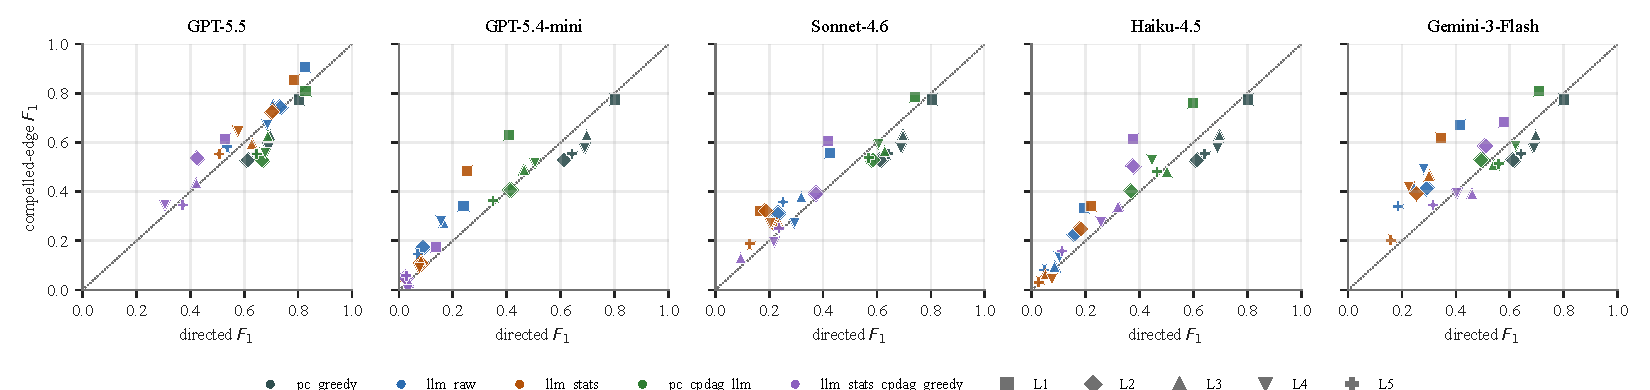
\includegraphics[width=\linewidth]{figures/generated/fig_e_score_axis_disagreement.pdf}
\caption{Compelled-edge $F_1$ versus directed $F_1$ per (level, method) cell, one sub-axis per model. Marker colour encodes method, marker shape encodes level. Diagonal: equal scores. Points above the diagonal correspond to submissions where the model orients the observationally identifiable (compelled) edges more reliably than the unrestricted directed set --- they get the easy oriented edges right but submit many extra wrong directions. Most strongly visible for \texttt{llm\_stats} on GPT-5.4-mini, Sonnet-4.6, and Haiku-4.5 (smaller models with the stats prompt produce orientation noise on top of correct compelled-edge inference).}
\label{fig:e-score-axis}
\end{figure}

The diagonal is the case where the two scores agree; cells well off the diagonal are where the score axes disagree on policy ranking, and that disagreement is the case for reporting both. \texttt{pc\_greedy} sits below the diagonal in every panel (compelled $<$ directed): the classical pipeline orients edges with the $z$-calibrated mean-shift rule applied uniformly, so directed $F_1$ benefits from correctly oriented non-compelled edges that compelled-$F_1$ does not credit. The opposite pattern --- compelled $>$ directed --- appears mostly for \texttt{llm\_stats} and \texttt{llm\_raw} on the smaller models, where the compelled fraction of submissions is more reliably oriented than the rest.

\begin{figure}[h]
\centering
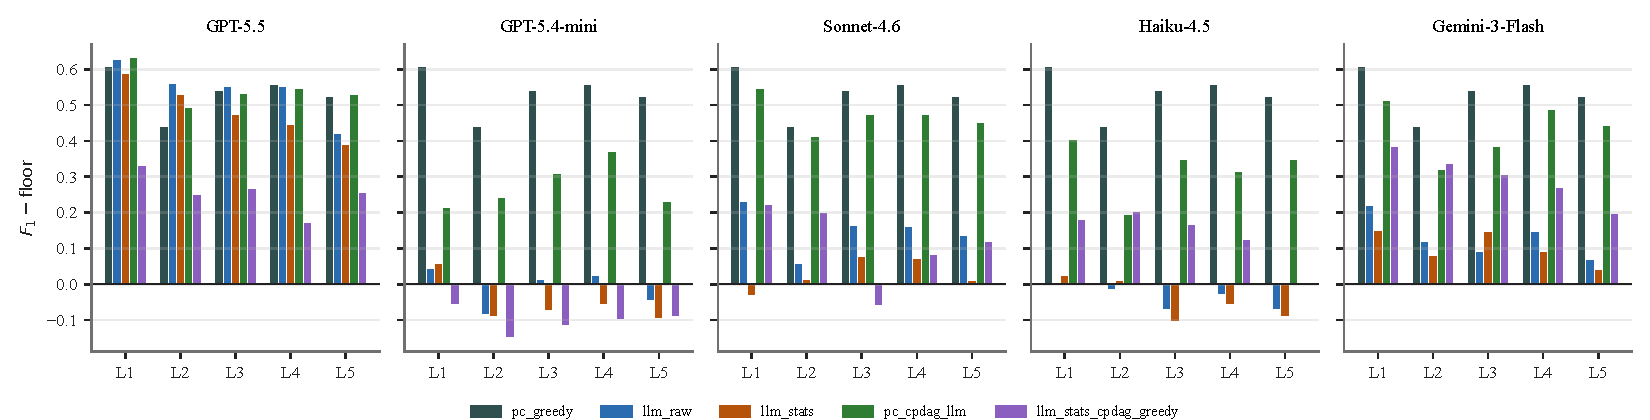
\includegraphics[width=\linewidth]{figures/generated/fig_e_gap_above_floor_by_level.pdf}
\caption{Gap above the random-submission directed-$F_1$ floor (Appendix~\ref{app:floor}) per level per method, one sub-axis per model. Zero is the floor. Bars below zero are submissions worse than uniform random at that density.}
\label{fig:e-gap-floor}
\end{figure}

This is the calibrated cross-model picture. The floor-subtracted view collapses the ladder dropoff that the raw $F_1$ tables make hard to read across rows of different density. Three shapes are visible: (i) GPT-5.5 keeps a near-flat $\sim 0.5$ gap across L1--L5 for the three competitive policies, (ii) Sonnet-4.6 and Gemini-3-Flash maintain positive gaps everywhere but lose ground on \texttt{llm\_raw} as $d$ grows, and (iii) GPT-5.4-mini and Haiku-4.5 produce sub-floor submissions on the end-to-end policies and only recover a positive gap with the CPDAG prior. The chart makes clear why the cross-model headline number averaged at L1--L5 is a poor summary: the spread within a model across levels is comparable to the spread across models at a single level.

\subsection{Cost and action counts}
\label{app:results:cost}

The active LLM policies differ in token volume by 2--3 orders of magnitude across models, with the smaller models compensating for low directed-$F_1$ output via low cost per submission. The table reports averages over L1--L5 of \texttt{cost\_usd\_mean} and \texttt{total\_actions\_mean} per cell, plus the directed-$F_1$-per-dollar ratio.

\begin{center}
\scriptsize
\setlength{\tabcolsep}{4.0pt}
\begin{tabular}{@{}l l c c c c@{}}
\toprule
Model & Method & cost (\$) & actions & dir $F_1$ & $F_1$ / \$ \\
\midrule
GPT-5.5         & \texttt{llm\_raw}                & $0.706$ & $5.0$  & $0.697$ & $0.99$ \\
                & \texttt{llm\_stats}              & $0.927$ & $10.4$ & $0.640$ & $0.69$ \\
                & \texttt{pc\_cpdag\_llm}          & $0.178$ & $3.8$  & $0.701$ & $3.95$ \\
                & \texttt{llm\_stats\_cpdag\_greedy} & $0.161$ & $5.8$  & $0.411$ & $2.56$ \\
\midrule
GPT-5.4-mini    & \texttt{llm\_raw}                & $0.015$ & $2.5$  & $0.145$ & $9.92$ \\
                & \texttt{llm\_stats}              & $0.015$ & $4.3$  & $0.103$ & $6.89$ \\
                & \texttt{pc\_cpdag\_llm}          & $0.005$ & $2.3$  & $0.429$ & $80.5$ \\
                & \texttt{llm\_stats\_cpdag\_greedy} & $0.009$ & $4.8$  & $0.053$ & $5.93$ \\
\midrule
Sonnet-4.6      & \texttt{llm\_raw}                & $0.191$ & $2.9$  & $0.305$ & $1.60$ \\
                & \texttt{llm\_stats}              & $0.056$ & $2.3$  & $0.183$ & $3.26$ \\
                & \texttt{pc\_cpdag\_llm}          & $0.058$ & $3.0$  & $0.626$ & $10.7$ \\
                & \texttt{llm\_stats\_cpdag\_greedy} & $0.670$ & $26.6$ & $0.268$ & $0.40$ \\
\midrule
Haiku-4.5       & \texttt{llm\_raw}                & $0.028$ & $3.0$  & $0.118$ & $4.20$ \\
                & \texttt{llm\_stats}              & $0.111$ & $12.3$ & $0.111$ & $0.99$ \\
                & \texttt{pc\_cpdag\_llm}          & $0.014$ & $2.8$  & $0.476$ & $34.3$ \\
                & \texttt{llm\_stats\_cpdag\_greedy} & $0.299$ & $35.0$ & $0.289$ & $0.97$ \\
\midrule
Gemini-3-Flash  & \texttt{llm\_raw}                & $0.025$ & $3.1$  & $0.284$ & $11.5$ \\
                & \texttt{llm\_stats}              & $0.125$ & $15.0$ & $0.257$ & $2.05$ \\
                & \texttt{pc\_cpdag\_llm}          & $0.010$ & $3.0$  & $0.585$ & $57.1$ \\
                & \texttt{llm\_stats\_cpdag\_greedy} & $0.173$ & $33.6$ & $0.454$ & $2.63$ \\
\bottomrule
\end{tabular}
\end{center}

The \texttt{pc\_cpdag\_llm} policy is consistently the cheapest active LLM policy per directed-$F_1$ point in every panel, often by an order of magnitude --- the LLM is not asked to recover the skeleton, only to orient a small set of undirected edges, so the prompt is shorter and the action count smaller. Two action-count outliers are worth noting. Sonnet-4.6 \texttt{llm\_stats\_cpdag\_greedy} averages $26.6$ actions per episode against the budget of $40$, and Haiku-4.5 \texttt{llm\_stats\_cpdag\_greedy} averages $35.0$ --- both saturate the stats budget with statistical queries and still produce a weaker submission than the $3$-action \texttt{pc\_cpdag\_llm} run on the same panel. Cost-per-$F_1$ is therefore not a soft proxy for capability: the policies that spend more on the stats path also score worse, on these models.
